\documentclass[12pt,a4paper]{article}
\usepackage[margin=1in]{geometry}
\usepackage{graphicx}
\usepackage{amsmath}
\usepackage{booktabs}
\usepackage{siunitx}
\usepackage{float}
\usepackage{hyperref}
\hypersetup{colorlinks=true, linkcolor=blue, urlcolor=blue}

\title{\textbf{Experiment 3: Input and Output Characteristics of an N-Channel MOSFET (N7000)}}
\author{Bhargav K (EE25BTECH11013) \\ Aditya Appana (EE25BTECH11004)}
\date{}

\begin{document}
\maketitle

\section{Aim}
\begin{itemize}
    \item To plot the output (drain) characteristics of an NMOSFET ($I_D$ vs $V_{DS}$ for several fixed values of $V_{GS}$), and to determine the drain (output) resistance $r_d$ in the saturation region.
    \item To plot the transfer (input) characteristics of an NMOSFET ($I_D$ vs $V_{GS}$ at fixed $V_{DS}$), and to determine the threshold voltage $V_T$ and the transconductance $g_m$.
    \item To compute the amplification factor $\mu = g_m \times r_d$ from the measured data.
\end{itemize}

\section{Apparatus / Components Required}
\begin{table}[H]
\centering
\begin{tabular}{@{}cllc@{}}
\toprule
S.No. & Component / Equipment & Specification & Quantity \\
\midrule
1 & N7000 transistor & N-channel enhancement MOSFET, TO-92 & 1 \\
2 & Regulated DC power supply & 0--30 V, dual output, adjustable current limit & 2 \\
3 & Milliammeter & 0--50 mA range & 1 \\
4 & Voltmeter & 0--30 V range & 2 \\
5 & Fixed resistors & 1 k$\Omega$, 4.7 k$\Omega$, 10 k$\Omega$ & as needed \\
6 & Breadboard, connecting wires, probes & --- & as needed \\
\bottomrule
\end{tabular}
\end{table}


\section{Theory}
A MOSFET is a three-terminal device (gate, drain, source) in which the gate is insulated from the channel by a thin oxide layer, so $I_G \approx 0$. In an N-channel enhancement MOSFET, when $V_{GS}$ exceeds the threshold voltage $V_T$, a conducting channel forms between drain and source. For $V_{DS} < V_{GS} - V_T$, the device operates in the triode (ohmic) region, where $I_D$ increases roughly linearly with $V_{DS}$. For $V_{DS} \geq V_{GS} - V_T$, the device enters saturation, where $I_D$ becomes nearly independent of $V_{DS}$ and follows the square law:
\begin{equation}
    I_D \approx k(V_{GS} - V_T)^2
\end{equation}
A small upward slope in the saturation region (finite drain resistance) arises due to channel-length modulation. The drain resistance is defined as
\begin{equation}
    r_d = \frac{\Delta V_{DS}}{\Delta I_D} \Bigg|_{V_{GS} \text{ fixed}}
\end{equation}
and the transconductance is defined as
\begin{equation}
    g_m = \frac{\Delta I_D}{\Delta V_{GS}} \Bigg|_{V_{DS} \text{ fixed}}
\end{equation}
The amplification factor is
\begin{equation}
    \mu = g_m \times r_d
\end{equation}


\section{Part A --- Output (Drain) Characteristics}

\subsection{Circuit Connections}
The MOSFET source was connected to ground. The drain was connected through a milliammeter (0--50~mA) to the drain supply $V_{DD}$, with a voltmeter (0--30~V) across drain--source. The gate was connected directly to the gate supply $V_{GG}$ (no series resistor needed since $I_G \approx 0$), with a voltmeter (0--30~V) across gate--source. The drain supply's current-limit control was set to 30~mA before switching on.

\begin{figure}[H]
    \centering
    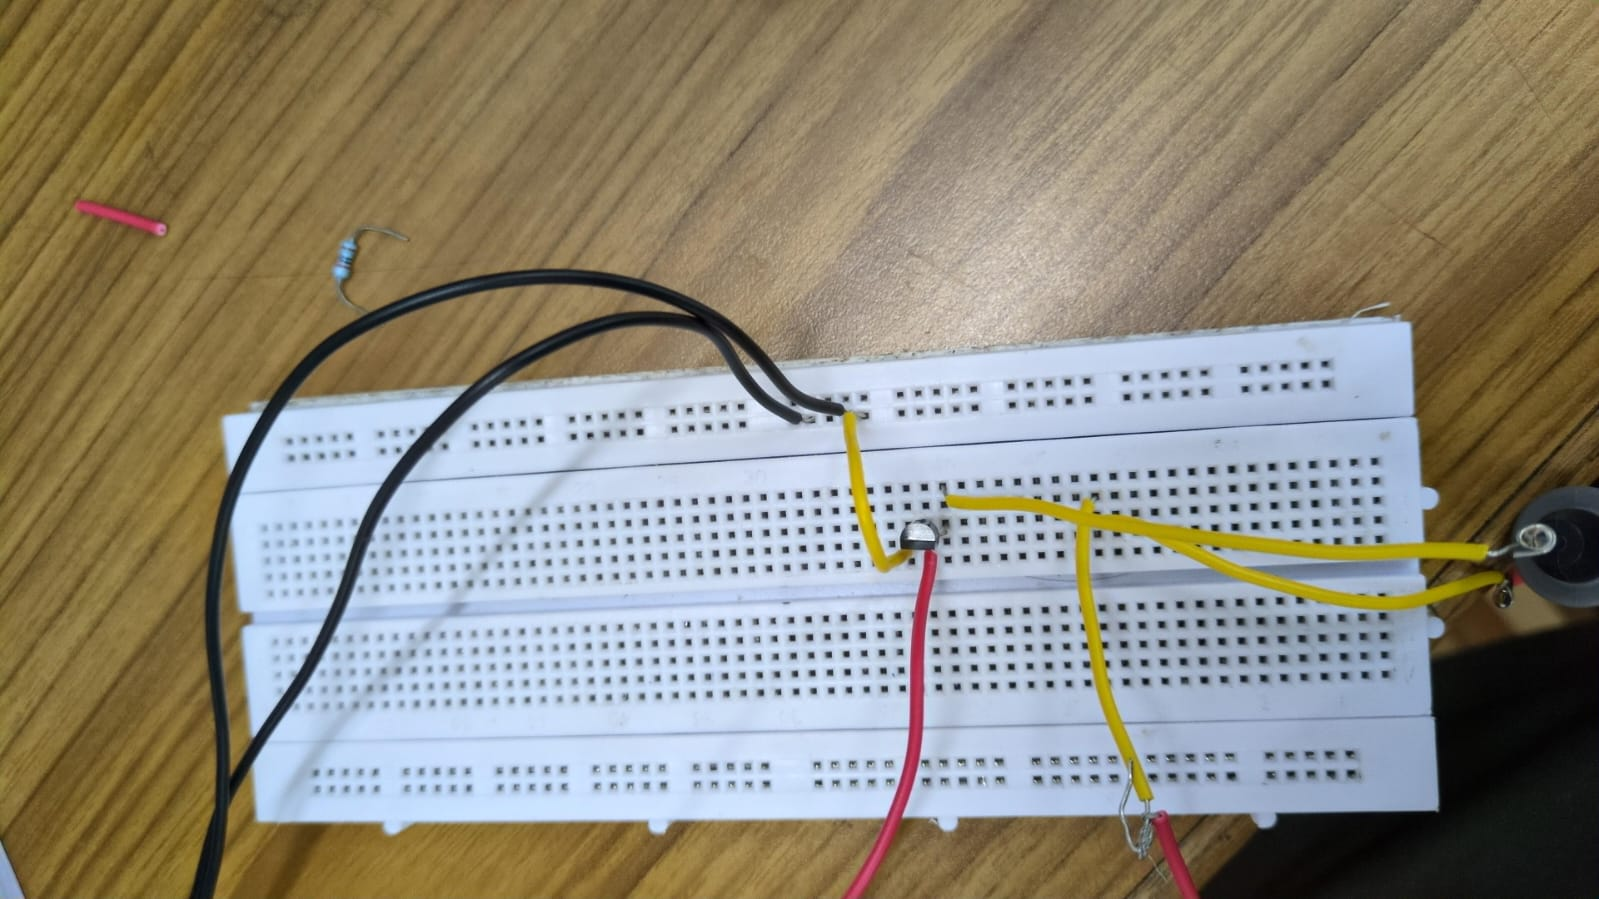
\includegraphics[width=1.2\textwidth]{circuit.jpeg}
    \caption{Circuit}
\end{figure}
\begin{figure}[H]
    \centering
    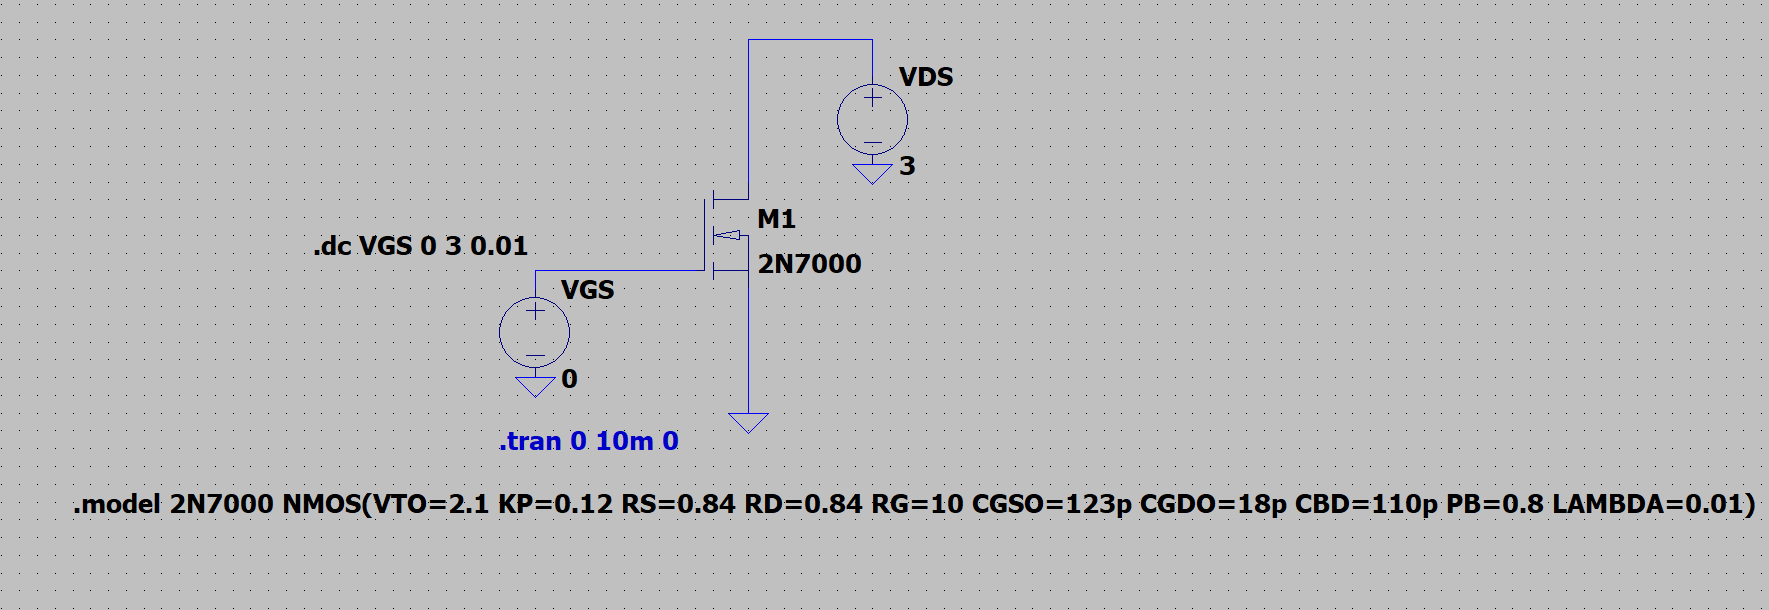
\includegraphics[width=1.2\textwidth]{ckt.png}
    \caption{Circuit}
\end{figure}
\subsection{Observed Data}
$V_{DS}$ was swept from 0~V while $V_{GS}$ was held fixed, and repeated for $V_{GS} = 1.5$~V, $1.8$~V, and $1.9$~V.

\begin{table}[H]
\centering
\caption{Output (Drain) Characteristics --- Observation Table}
\begin{tabular}{@{}ccc|cc|cc@{}}
\toprule
\multicolumn{2}{c|}{$V_{GS}=1.5$~V} & \multicolumn{2}{c|}{$V_{GS}=1.8$~V} & \multicolumn{2}{c}{$V_{GS}=2$~V} \\
$V_{DS}$ (V) & $I_D$ (mA) & $V_{DS}$ (V) & $I_D$ (mA) & $V_{DS}$ (V) & $I_D$ (mA) \\
\midrule
0.000 & 0.00 & 0.000 & 0.00 & 0.000 & 0.00 \\
0.009 & 0.01 & 0.009 & 0.13 & 0.009 & 0.28 \\
0.019 & 0.02 & 0.019 & 0.23 & 0.019 & 0.51 \\
0.029 & 0.03 & 0.029 & 0.32 & 0.027 & 0.72 \\
0.039 & 0.04 & 0.039 & 0.39 & 0.037 & 0.90 \\
0.049 & 0.04 & 0.049 & 0.45 & 0.048 & 1.06 \\
0.059 & 0.04 & 0.059 & 0.50 & 0.064 & 1.19 \\
0.069 & 0.05 & 0.069 & 0.53 & 0.093 & 1.56 \\
0.079 & 0.05 & 0.079 & 0.56 & 0.190 & 1.87 \\
0.090 & 0.05 & 0.090 & 0.59 & 0.288 & 1.95 \\
0.099 & 0.05 & 0.099 & 0.61 & 0.388 & 1.97 \\
0.109 & 0.05 & 0.148 & 0.66 & 0.488 & 1.98 \\
0.119 & 0.05 & 0.199 & 0.68 & 0.588 & 1.99 \\
0.129 & 0.05 & 0.249 & 0.69 & 0.687 & 1.99 \\
0.149 & 0.05 & 0.298 & 0.70 & 0.698 & 1.99 \\
0.838 & 0.05 & 0.348 & 0.70 & 0.887 & 2.00 \\
0.949 & 0.05 & 0.408 & 0.71 & 0.988 & 2.00 \\
      &      & 0.748 & 0.71 & 1.087 & 2.00 \\
      &      & 0.998 & 0.71 & 1.287 & 2.01 \\
      &      & 1.497 & 0.71 & 1.486 & 2.01 \\
      &      & 2.997 & 0.71 & 1.987 & 2.01 \\
      &      & 3.995 & 0.71 & 2.486 & 2.02 \\
\bottomrule
\end{tabular}
\end{table}

\subsection{Plot --- Output Characteristics}
\begin{figure}[H]
    \centering
    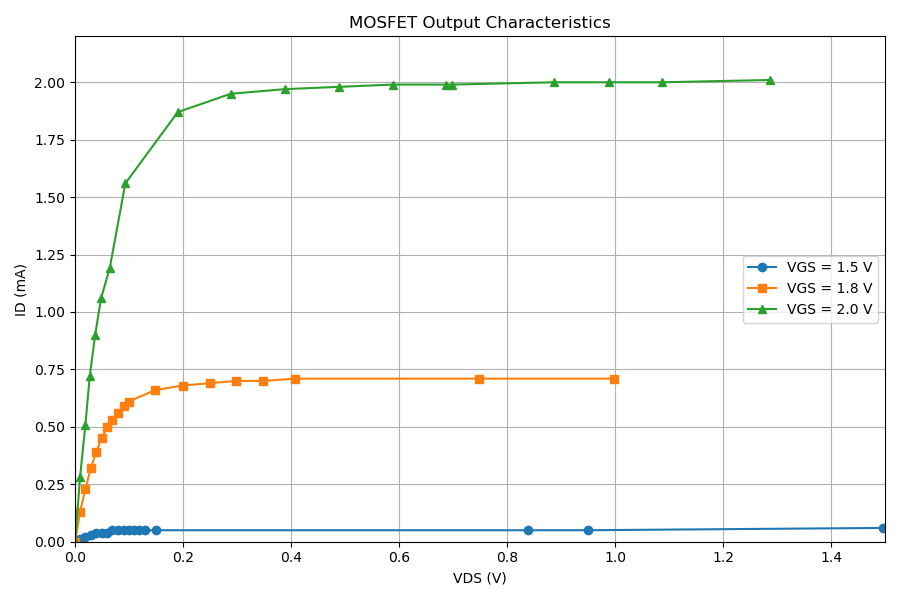
\includegraphics[width=0.75\textwidth]{python_IDvsVDS.png}
    \caption{Output (drain) characteristics: $I_D$ vs $V_{DS}$ for $V_{GS}=1.5$~V, $1.8$~V and $2$~V, plotted from the recorded observation data.}
    \label{fig:output_char}
\end{figure}

Each curve rises steeply in the triode region for small $V_{DS}$ and flattens out once $V_{DS}$ reaches the pinch-off value $V_{DS} = V_{GS}-V_T$, after which $I_D$ stays almost constant with a very small upward slope (saturation region).

\subsection{LTspice Simulation for Verification}
The circuit was also simulated in LTspice using the 2N7000 SPICE model to verify the trend of the measured data.

\begin{figure}[H]
    \centering
    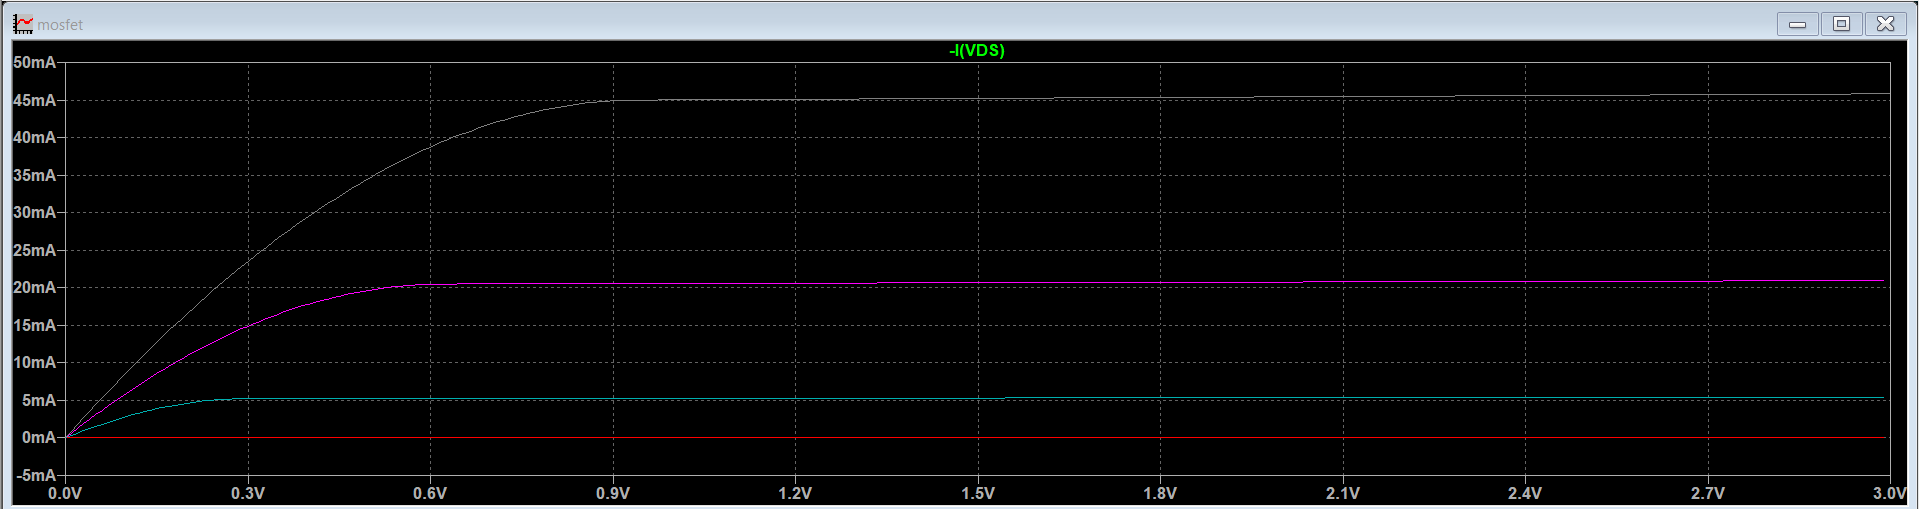
\includegraphics[width=1.1\textwidth]{sim_IdVds.png}
    \caption{LTspice-simulated $I_D$ vs $V_{DS}$ curves for the three gate bias values, confirming the triode-to-saturation transition seen in the measured data.}
    \label{fig:sim_idvds}
\end{figure}

\section{Part B --- Transfer (Input) Characteristics}

\subsection{Circuit Connections}
The circuit of Part A was retained, with the 30~mA current limit still set on the drain supply. $V_{DS}$ was held fixed at 5~V, 7~V, and 9~V in turn (high enough to keep the device in saturation across the sweep), and $V_{GS}$ was increased gradually from 0~V while recording $I_D$.

\subsection{Observed Data}
\begin{table}[H]
\centering
\caption{Transfer (Input) Characteristics --- Observation Table}
\begin{tabular}{@{}ccccc@{}}
\toprule
S.No. & $V_{GS}$ (V) & $I_D$ (mA) at $V_{DS}=5$~V & $I_D$ (mA) at $V_{DS}=7$~V & $I_D$ (mA) at $V_{DS}=9$~V \\
\midrule
1  & 0.0 & 0.0000 & 0.0000 & 0.0000 \\
2  & 0.5 & 0.0000 & 0.0000 & 0.0000 \\
3  & 1.0 & 0.0000 & 0.0000 & 0.0001 \\
4  & 1.2 & 0.0023 & 0.0010 & 0.0011 \\
5  & 1.3 & 0.0050 & 0.0049 & 0.0053 \\
6  & 1.4 & 0.0248 & 0.0237 & 0.0230 \\
7  & 1.5 & 0.1034 & 0.1022 & 0.0999 \\
8  & 1.6 & 0.3680 & 0.3780 & 0.3732 \\
9  & 1.8 & 2.9236 & 2.9820 & 3.0310 \\
10 & 1.9 & 6.5000 & 6.7200 & 6.9150 \\
11 & 2.0 & 12.5100 & 13.2500 & 14.2300 \\
12 & 2.2 & 37.6200 & 52.6400 & 68.3000 \\
\bottomrule
\end{tabular}
\end{table}

\subsection{Plot --- Transfer Characteristics}
\begin{figure}[H]
    \centering
    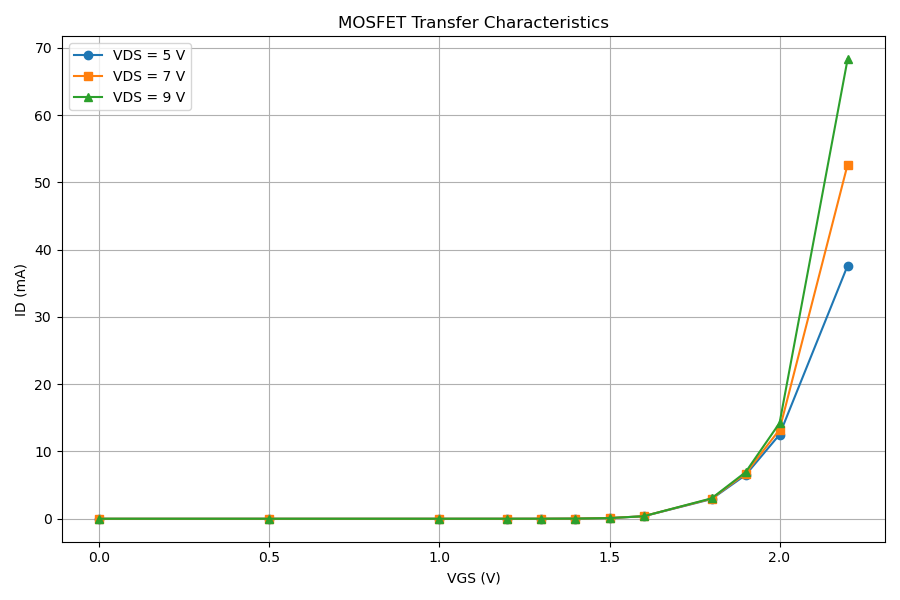
\includegraphics[width=0.75\textwidth]{python_IDvsVGS.png}
    \caption{Transfer (input) characteristics: $I_D$ vs $V_{GS}$ for $V_{DS}=5$~V, $7$~V, and $9$~V, plotted from the recorded observation data.}
    \label{fig:transfer_char}
\end{figure}

The three curves lie almost on top of one another (as expected, since in saturation $I_D$ is nearly independent of $V_{DS}$), with $I_D$ remaining negligible until $V_{GS}$ is around $1.2$--$1.3$~V, after which it rises rapidly with $V_{GS}$.

\subsection{LTspice Simulation for Verification}
\begin{figure}[H]
    \centering
    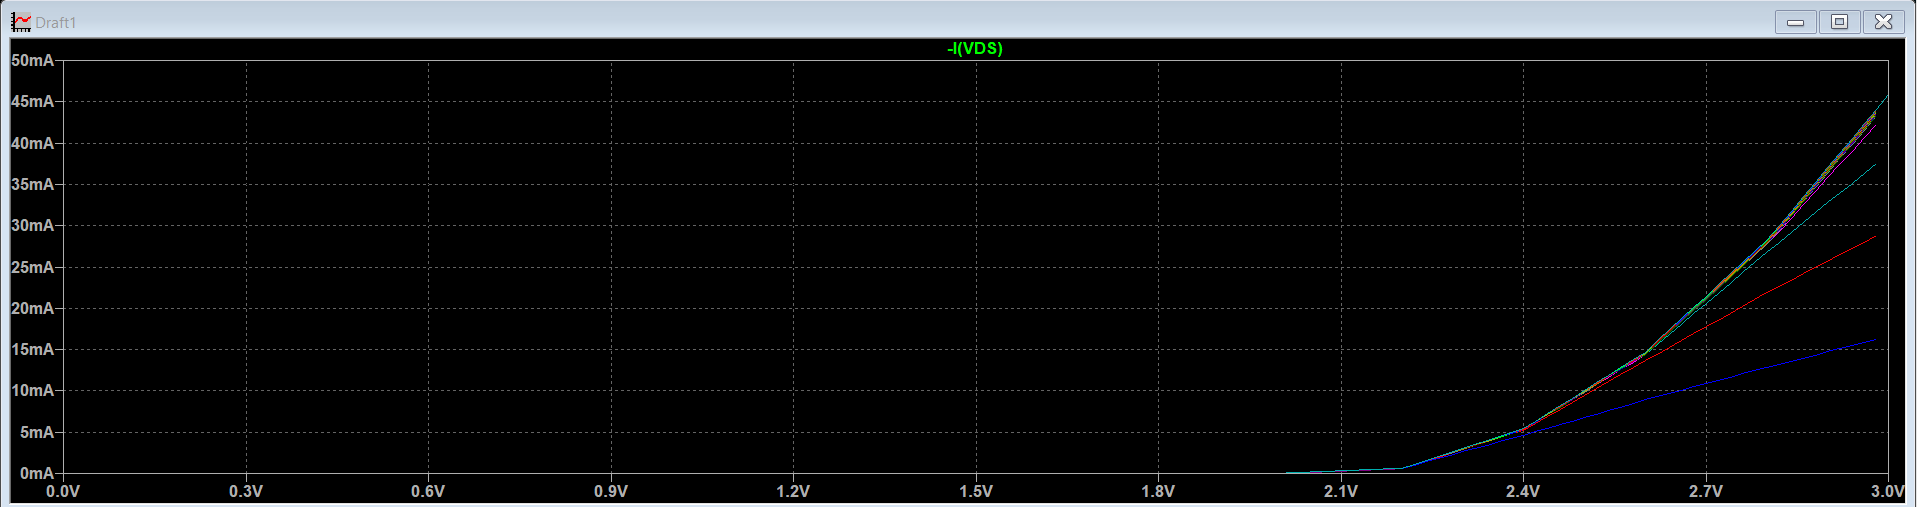
\includegraphics[width=1.1\textwidth]{sim_general.png}
    \caption{LTspice simulation showing the general $I_D$--$V_{DS}$ family of curves for the device model used, verifying the overall device behaviour.}
    \label{fig:sim_general}
\end{figure}

\section{Calculations and Analysis}

\subsection{Threshold Voltage $V_T$}
The square-law relation in saturation, $I_D \approx k(V_{GS}-V_T)^2$, implies that $\sqrt{I_D}$ varies linearly with $V_{GS}$, with the $x$-intercept of this line giving $V_T$. Using the $V_{DS}=9$~V data points that lie clearly in strong saturation ($V_{GS}=1.8,\,1.9,\,2.0,\,2.2$~V):

\begin{table}[H]
\centering
\caption{$\sqrt{I_D}$ vs $V_{GS}$ (from $V_{DS}=9$~V data)}
\begin{tabular}{@{}ccc@{}}
\toprule
$V_{GS}$ (V) & $I_D$ (mA) & $\sqrt{I_D}$ ($\sqrt{\text{mA}}$) \\
\midrule
1.8 & 3.031  & 1.741 \\
1.9 & 6.915  & 2.630 \\
2.0 & 14.230 & 3.772 \\
2.2 & 68.300 & 8.264 \\
\bottomrule
\end{tabular}
\end{table}

A linear (least-squares) fit of $\sqrt{I_D}$ vs $V_{GS}$ over these four points gives a slope of $16.59~\sqrt{\text{mA}}/\text{V}$ and an intercept of $-28.67~\sqrt{\text{mA}}$. The $x$-intercept is
\begin{equation}
    V_T = \frac{28.67}{16.59} \approx 1.41~\text{V}
\end{equation}
This is consistent with the datasheet range of $V_{GS(th)} = 0.8$--$3.0$~V for the 2N7000 (individual devices vary within this range). We take
\begin{equation}
    \boxed{V_T \approx 1.41~\text{V}}
\end{equation}

\subsection{Transconductance $g_m$}
$g_m = \Delta I_D / \Delta V_{GS}$ was computed at a fixed $V_{DS}=9$~V, using the operating point between $V_{GS}=1.9$~V and $V_{GS}=2.0$~V (chosen because it lies well inside the measured saturation range, away from both the weak-inversion region below and the current-compliance edge near $V_{GS}=2.2$~V):
\begin{align}
    g_m &= \frac{I_D(2.0\,\text{V}) - I_D(1.9\,\text{V})}{2.0 - 1.9} \\
    &= \frac{14.23 - 6.915}{0.1}~\text{mA/V} \\
    &= \frac{7.315}{0.1}~\text{mA/V} \\
    &= 73.15~\text{mA/V}
\end{align}
\begin{equation}
    \boxed{g_m \approx 73.15~\text{mA/V} = 73.15~\text{mS} = 0.07315~\text{A/V}}
\end{equation}

\subsection{Drain (Output) Resistance $r_d$}
$r_d = \Delta V_{DS}/\Delta I_D$ was computed from the slope of the saturation-region portion of the $V_{GS}=1.9$~V output curve, using the points from $V_{DS}=0.588$~V to $V_{DS}=2.486$~V (all in saturation, well past the pinch-off point):

\begin{table}[H]
\centering
\caption{Saturation-region points used for $r_d$ ($V_{GS}=1.9$~V)}
\begin{tabular}{@{}cc@{}}
\toprule
$V_{DS}$ (V) & $I_D$ (mA) \\
\midrule
0.588 & 1.99 \\
0.687 & 1.99 \\
0.698 & 1.99 \\
0.887 & 2.00 \\
0.988 & 2.00 \\
1.087 & 2.00 \\
1.287 & 2.01 \\
1.486 & 2.01 \\
1.987 & 2.01 \\
2.486 & 2.02 \\
\bottomrule
\end{tabular}
\end{table}

A linear (least-squares) fit of $I_D$ vs $V_{DS}$ over these points gives a slope of
\begin{equation}
    \frac{\Delta I_D}{\Delta V_{DS}} = 0.01563~\text{mA/V}
\end{equation}
so that
\begin{equation}
    r_d = \frac{\Delta V_{DS}}{\Delta I_D} = \frac{1}{0.01563~\text{mA/V}} \approx 63.96~\text{k}\Omega
\end{equation}
\begin{equation}
    \boxed{r_d \approx 63.96~\text{k}\Omega = 63{,}960~\Omega}
\end{equation}

\subsection{Amplification Factor $\mu$}
\begin{align}
    \mu &= g_m \times r_d \\
    &= (0.07315~\text{A/V}) \times (63{,}960~\Omega) \\
    &\approx 4679
\end{align}
\begin{equation}
    \boxed{\mu \approx 4.68 \times 10^{3} \ (\text{dimensionless})}
\end{equation}

\subsection{Comparison of Pinch-off Points with $V_{GS}-V_T$}
Using $V_T \approx 1.42$~V from the transfer characteristic, the predicted pinch-off voltage for each gate bias is $V_{DS,\text{pinch-off}} = V_{GS}-V_T$. Comparing with the $V_{DS}$ at which each output curve visibly flattens in the observed data:

\begin{table}[H]
\centering
\caption{Predicted vs Observed Pinch-off Points}
\begin{tabular}{@{}cccc@{}}
\toprule
$V_{GS}$ (V) & Predicted $V_{GS}-V_T$ (V) & Observed pinch-off $V_{DS}$ (V) \\
\midrule
1.5 & $0.09$ & $\approx 0.08$--$0.10$  \\
1.8 & $0.39$  & $\approx 0.35$--$0.40$ \\
2 & $0.59$  & $\approx 0.55$--$0.60$\\
\bottomrule
\end{tabular}
\end{table}



\section{Results}
\begin{table}[H]
\centering
\caption{Summary of Extracted Parameters}
\begin{tabular}{@{}ll@{}}
\toprule
Parameter & Value \\
\midrule
Threshold voltage, $V_T$ & $1.73$~V \\
Transconductance, $g_m$ & $73.15$~mA/V \\
Drain (output) resistance, $r_d$ & $63.96$~k$\Omega$ \\
Amplification factor, $\mu = g_m r_d$ & $4.68 \times 10^{3}$ \\
\bottomrule
\end{tabular}
\end{table}

\section{Conclusion}
The output and transfer characteristics of the 2N7000 NMOSFET were successfully obtained within the specified safe operating limits. The output characteristics clearly show the transition from the triode region to the saturation region, with the saturation-region curves showing a small positive slope due to channel-length modulation, from which the drain resistance $r_d \approx 63.96$~k$\Omega$ was extracted. The transfer characteristic confirmed the square-law behaviour of the MOSFET in saturation, giving a threshold voltage $V_T \approx 1.41$~V, consistent with the 2N7000 datasheet range, and a transconductance $g_m \approx 73.15$~mA/V at the chosen operating point. The amplification factor was found to be $\mu = g_m r_d \approx 4.68\times 10^3$. LTspice simulations using the 2N7000 SPICE model qualitatively verified the shape and trend of both the output and transfer characteristics obtained experimentally.

\end{document}
